\subsection{The Halo Model Basics}

At the core of the halo model is the approximation that we can fully describe the complex structure of the cosmic web simply as a sum of its individual components: dark matter, gas, and galaxies, all distributed in haloes. Fig. \ref{fig:halo} shows the schematic of the halo model approach.

\begin{figure}[htpb]
    \centering
    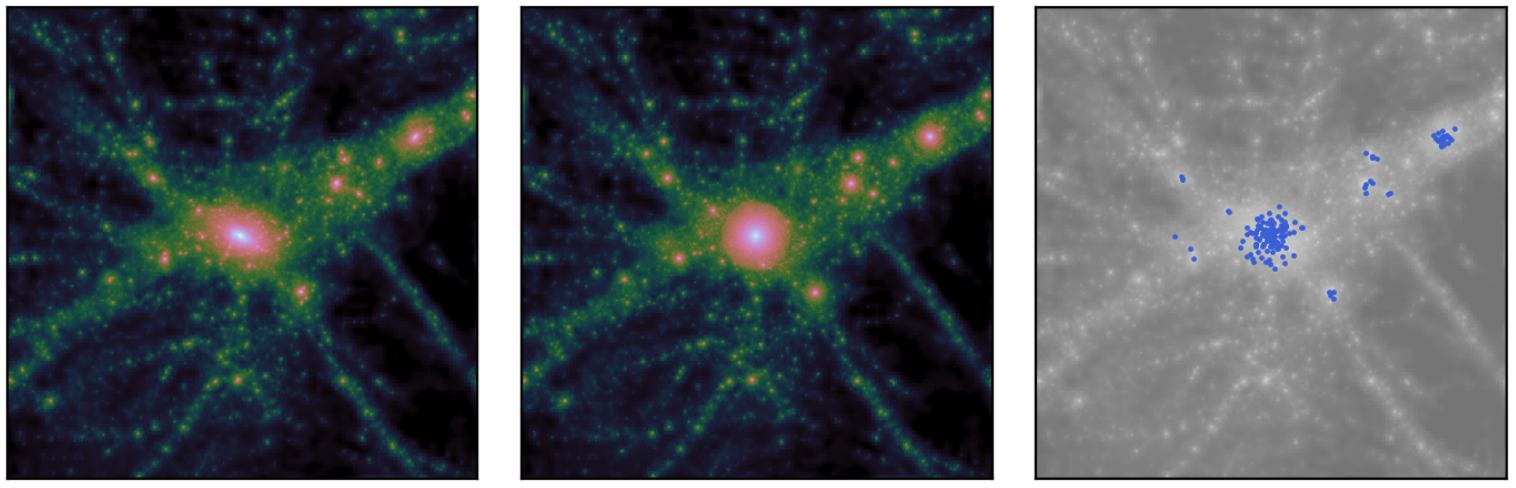
\includegraphics[scale=0.2]{img/halo.png}
    \caption{A schematic visualization of the halo model process. The left-hand panel shows the matter density field of an $N$-body simulation. The central panel shows the result of isolating all haloes identified in the simulation and replacing them with idealized spherical haloes of the same mass. The right-hand panel shows the result of populating these haloes with galaxies according to a simple galaxy-occupation prescription.}
    \label{fig:halo}
\end{figure}

We start by defining a field in the real space, $\theta_u(\bm{x})$, where $\bm{x}$ is the three-dimensional comoving position and the label $u$ stands for the field we are interested in modeling; this could be matter, halo, or galaxy over-densities. We make the assumption that everything in our field is contained within haloes distributed throughout the space with a spherically symmetric profile, $W_{u, i}$, centered at position $\bm{x}_i$, such that
\begin{equation}
    \theta_u(\bm{x}) = \sum_i N_i W_{u, i}\left(|\bm{x} - \bm{x}_i|\right)
    \label{eq:1}
\end{equation}
where the sum runs over all volume elements and $N_i = \{0, 1\}$ determines whether there is a halo center in that volume element. The Fourier transform of the field, in terms of comoving wavenumber $\bm{k}$, is given by
\begin{align}
    \label{eq:2}
    \hat{\theta}_u(\bm{k}) &= \int \theta_u(\bm{x}) e^{-i\bm{k}\cdot\bm{x}} d^3\bm{x} \\
    &= \int  \sum_i N_i W_{u, i}\left(|\bm{x} - \bm{x}_i|\right) e^{-i\bm{k}\cdot\bm{x}} d^3\bm{x} \\
    &= \sum_i N_i e^{- i\bm{k} \cdot \bm{x}_i} \int W_{u, i}(|\bm{r}|) e^{-i |\bm{k}| |\bm{r}| \cos\theta} d^3\bm{r} \\
    &= \sum_i N_i e^{- i\bm{k} \cdot \bm{x}_i} 2\pi \int_0^\infty \int_0^\pi W_{u, i}(|\bm{r}|) e^{-i |\bm{k}| |\bm{r}| \cos\theta} r^2 \sin\theta d\theta dr \\
    &= \sum_i N_i e^{- i\bm{k} \cdot \bm{x}_i} \int_0^\infty \frac{\sin(kr)}{kr} W_{u, i}(r) 4\pi r^2 dr = \sum_i N_i e^{-i \bm{k} \cdot \bm{x}_i} \hat{W}_{u, i}(k).
    \label{eq:field}
\end{align}
We assume that the properties of each halo $i$ are defined solely by its mass $M_i$, such that $W_{u, i} = W_u(M_i, r)$ and that the halo masses are distributed according to the halo-mass-distribution function $n(M)$, where $n(M) dM$ is the number of density of haloes with masses between $M$ and $M+dM$. Using this, we can find the mean value of $\theta_u(\bm{x})$ by averaging over all haloes,
\begin{align}
    \langle\theta_u(\bm{x})\rangle &= \left\langle\sum_iN_iW_u(M_i, |\bm{x} - \bm{x}_i|)\right\rangle\\
    &= \sum_i\left\langle N_iW_u(M_i, |\bm{x} - \bm{x}_i|)\right\rangle\\
    &= \sum_i \int_0^\infty dM n(M) \Delta V_i  W_u(M, |\bm{x} - \bm{x}_i) \\
    &= \int_0^\infty dM n(M) \int d^3 \bm{x}' W_u(M, |\bm{x} - \bm{x}') \\
    &= \int_0^\infty dM n(M) \int d^3 \bm{x}' W_u(M) U_u(M, |\bm{x} - \bm{x}') \\
    &= \int_0^\infty dM W_u(M) n(M),
\end{align}
where $U_u(M, x)$ is the normalized halo profile. We can define $\hat{W}_u(M, k) = W_u(M)\hat{U}_u(M, k)$. Since $U_u(M, x)$ is the normalized profile, this implies that $\hat{W}_u(M, k\to0) = \hat{W}_u(M)$. We can understand this by considering that at large scales a halo acts as a point mass, which translates to a constant in Fourier space.

We consider the correlation function between the two fields $\theta_u$ and $\theta_v$, which could be identical or different. Our fields are real, isotropic, and homogeneous such that
\begin{equation}
    \langle\theta_u(\bm{x})\theta_v(\bm{x}')\rangle = \xi_{uv}(|\bm{x} - \bm{x}'|),
\end{equation}
where $\xi_{uv}$ is the two-point correlation function and it only depends on the separation. In Fourier space, we have the power spectrum,
\begin{equation}
    \langle\hat{\theta}_u(\bm{k})\hat{\theta}^*_v(\bm{k}')\rangle = (2\pi)^3 \delta_D(\bm{k}-\bm{k}')P_{uv}(k),
\end{equation}
where $\delta_D$ is the Dirac delta function. The dimension of the power spectrum is volume times the dimensions of $\theta_u$ and $\theta_v$. If we want to remove the dependence on a volume dimension we can use,
\begin{equation}
    \Delta^2_{uv}(k) = 4\pi \left(\frac{k}{2\pi}\right)^3 P_{uv}(k).
\end{equation}
We can compute the power spectrum by inserting the fields from equation \ref{eq:field},
\begin{equation}
    \langle\hat{\theta}_u(\bm{k})\hat{\theta}^*_v(\bm{k}')\rangle = \left\langle\sum_{i,j} N_i N_j e^{-i \bm{k} \cdot \bm{x}_i} e^{i \bm{k}' \cdot \bm{x}_j} \hat{W}_{u, i}(k) \hat{W}_{v, j}(k')\right\rangle.
\end{equation}
We can separate the sums above into two parts: when $i=j$, we measure the field correlations within a single halo, the \emph{one-halo} term; when $i\neq j$, we measure field correlations between distinct haloes, called the \emph{two-halo} term.

The one-halo term is given by
\begin{equation}
    \langle\hat{\theta}_u(\bm{k})\hat{\theta}^*_v(\bm{k}')\rangle = \left\langle\sum_i N_i e^{-i (\bm{k} - \bm{k}') \cdot \bm{x}_i} \hat{W}_{u, i}(k) \hat{W}_{v, i}(k')\right\rangle,
    \label{eq:onehalo}
\end{equation}
where we used $N_i = N_i^2$. Take similar steps to what was done in finding the ensemble average of the field and the sum into continuous integrals,
\begin{align}
    \langle\hat{\theta}_u(\bm{k})\hat{\theta}^*_v(\bm{k}')\rangle &= \left\langle\sum_i N_i e^{-i (\bm{k} - \bm{k}') \cdot \bm{x}_i} \hat{W}_{u, i}(k) \hat{W}_{v, i}(k')\right\rangle \\
    &= \sum_i\left\langle\ N_i e^{-i (\bm{k} - \bm{k}') \cdot \bm{x}_i} \hat{W}_{u, i}(k) \hat{W}_{v, i}(k')\right\rangle\\
    &= \sum_i \int dM n(M) \Delta V_i e^{-i (\bm{k} - \bm{k}') \cdot \bm{x}_i} \hat{W}_{u, i}(k) \hat{W}_{v, i}(k')\\
    &= \int dM n(M) \int d^3\bm{x} e^{-i (\bm{k} - \bm{k}') \cdot \bm{x}_i} \hat{W}_{u}(k) \hat{W}_{v}(k')\\
    &= (2\pi)^3\delta_D(\bm{k} - \bm{k}') \int dM n(M) \hat{W}_{u}(k) \hat{W}_{v}(k'),
\end{align}
thus the one-halo power spectrum is,
\begin{equation}
    \label{eq:onehalop}
    P^{1h}_{uv}(k) = \int_0^\infty \hat{W}_{u, i}(M, k) \hat{W}_{v, i}(M, k) n(M) dM.
\end{equation}
The $k\to0$ limit of the one-halo term is independent of the shape of the halo profile. For this reason at large scales, the one-halo term only contributes a constant $P(k)$, so-called shot noise.

The two-halo term is defined when $i\neq j$. For this term, we have to consider the correlation between positions of haloes, $\langle N_iN_j\rangle = \xi^{ij}_{hh}(|\bm{x}_i - \bm{x}_j|)$.

\begin{align}
    \label{eq:twohalo}
    \langle\hat{\theta}_u(\bm{k})\hat{\theta}^*_v(\bm{k}')\rangle &= \left\langle\sum_i\sum_{i\neq j    } N_i N_j e^{-i \bm{k} \cdot \bm{x}_i} e^{i \bm{k}' \cdot \bm{x}_j} \hat{W}_{u, i}(M_1, k) \hat{W}_{v, j}(M_2, k')\right\rangle \\
    &= \sum_i\sum_{i\neq j}\left\langle\ N_i N_j e^{-i \bm{k} \cdot \bm{x}_i} e^{i \bm{k}' \cdot \bm{x}_j} \hat{W}_{u, i}(M_1, k) \hat{W}_{v, j}(M_2, k')\right\rangle \\
    &= \sum_i \sum_{i\neq j} \int dM_1 \int dM_2 n(M_1) n(M_2) \\
    &\nonumber \quad\quad\quad\quad\quad\quad\quad\Delta V_i \Delta V_j e^{-i \bm{k} \cdot \bm{x}_i} e^{i \bm{k}' \cdot \bm{x}_j} \hat{W}_{u, i}(M_1, k) \hat{W}_{v, j}(M_2, k')\\
    &= \int_0^\infty dM_1 \int_0^\infty dM_2~ n(M_1) n(M_2)  \hat{W}_{u}(M_1, k) \hat{W}_{v}(M_2, k') \\ \nonumber &\times \int d^3\bm{x} e^{-i \bm{k}\cdot \bm{x}} \int d^3\bm{x}' e^{i \bm{k'}\cdot \bm{x}'} \langle N(M_1, \bm{x}) N(M_2, \bm{x}')\rangle.
\end{align}
The last integral is 
\begin{equation}
    \int d^3\bm{x} e^{-i \bm{k}\cdot \bm{x}} \int d^3\bm{x}' e^{i \bm{k'}\cdot \bm{x}'} \langle N(M_1, \bm{x}) N(M_2, \bm{x}')\rangle = \langle \hat{N}(M_1, \bm{k}) \hat{N}^*(M_2, \bm{k}')\rangle = (2\pi)^3 \delta_D(\bm{k} - \bm{k}') P_{hh}(M_1, M_2, k),
\end{equation}
where $P_{hh}$ is the power spectrum of the halo centers with the shot-noise contribution subtracted. Thus, the two-halo power spectrum is
\begin{equation}
    P_{uv}^{2h}(k) = \int_0^\infty dM_1 \int_0^\infty dM_2~ n(M_1) n(M_2)  \hat{W}_{u}(M_1, k) \hat{W}_{v}(M_2, k') P_{hh}(M_1, M_2, k).
\end{equation}
As haloes are biased tracers of the underlying matter field, we can approximate the power spectrum of the halo centers as
\begin{equation}
    P_{hh}(M_1, M_2, k) = b(M_1)b(M_2)P_{mm}^{lin}(k)[1 + \beta^{nl}(M_1, M_2, k)],
\end{equation}
where $b(M)$ is the linear bias of haloes with mass $M$. The function $\beta^{nl}$ models all non-linear effects that are missing from the linear-bias-linear-field model, vanishing on large-scales: $\beta^{nl}(M_1, M_2, k\to0) = 0$. We can then write the two-halo power spectrum as
\begin{equation}
    P^{2h}_{uv}(k) = P^{lin}_{mm}(k)I^{nl}_{uv}(k) + P^{lin}_{mm}(k) \prod_{n=u, v} \left[\int_0^\infty \hat{W}_n(M, k) b(M) n(M) dM\right].
\end{equation}
It is common to set $I_{uv}^{nl}(k) = 0$ for all $k$ and therefore assume that halo bias is linear. 